% Options for packages loaded elsewhere
\PassOptionsToPackage{unicode}{hyperref}
\PassOptionsToPackage{hyphens}{url}
%
\documentclass[
  letterpaper,
]{scrartcl}
\title{2. Navigating the CMR-STAC API}
\author{}
\date{}

\usepackage{amsmath,amssymb}
\usepackage{lmodern}
\usepackage{iftex}
\ifPDFTeX
  \usepackage[T1]{fontenc}
  \usepackage[utf8]{inputenc}
  \usepackage{textcomp} % provide euro and other symbols
\else % if luatex or xetex
  \usepackage{unicode-math}
  \defaultfontfeatures{Scale=MatchLowercase}
  \defaultfontfeatures[\rmfamily]{Ligatures=TeX,Scale=1}
\fi
% Use upquote if available, for straight quotes in verbatim environments
\IfFileExists{upquote.sty}{\usepackage{upquote}}{}
\IfFileExists{microtype.sty}{% use microtype if available
  \usepackage[]{microtype}
  \UseMicrotypeSet[protrusion]{basicmath} % disable protrusion for tt fonts
}{}
\makeatletter
\@ifundefined{KOMAClassName}{% if non-KOMA class
  \IfFileExists{parskip.sty}{%
    \usepackage{parskip}
  }{% else
    \setlength{\parindent}{0pt}
    \setlength{\parskip}{6pt plus 2pt minus 1pt}}
}{% if KOMA class
  \KOMAoptions{parskip=half}}
\makeatother
\usepackage{xcolor}
\IfFileExists{xurl.sty}{\usepackage{xurl}}{} % add URL line breaks if available
\IfFileExists{bookmark.sty}{\usepackage{bookmark}}{\usepackage{hyperref}}
\hypersetup{
  pdftitle={2. Navigating the CMR-STAC API },
  hidelinks,
  pdfcreator={LaTeX via pandoc}}
\urlstyle{same} % disable monospaced font for URLs
\usepackage{color}
\usepackage{fancyvrb}
\newcommand{\VerbBar}{|}
\newcommand{\VERB}{\Verb[commandchars=\\\{\}]}
\DefineVerbatimEnvironment{Highlighting}{Verbatim}{commandchars=\\\{\}}
% Add ',fontsize=\small' for more characters per line
\newenvironment{Shaded}{}{}
\newcommand{\AlertTok}[1]{\textcolor[rgb]{1.00,0.00,0.00}{\textbf{#1}}}
\newcommand{\AnnotationTok}[1]{\textcolor[rgb]{0.38,0.63,0.69}{\textbf{\textit{#1}}}}
\newcommand{\AttributeTok}[1]{\textcolor[rgb]{0.49,0.56,0.16}{#1}}
\newcommand{\BaseNTok}[1]{\textcolor[rgb]{0.25,0.63,0.44}{#1}}
\newcommand{\BuiltInTok}[1]{#1}
\newcommand{\CharTok}[1]{\textcolor[rgb]{0.25,0.44,0.63}{#1}}
\newcommand{\CommentTok}[1]{\textcolor[rgb]{0.38,0.63,0.69}{\textit{#1}}}
\newcommand{\CommentVarTok}[1]{\textcolor[rgb]{0.38,0.63,0.69}{\textbf{\textit{#1}}}}
\newcommand{\ConstantTok}[1]{\textcolor[rgb]{0.53,0.00,0.00}{#1}}
\newcommand{\ControlFlowTok}[1]{\textcolor[rgb]{0.00,0.44,0.13}{\textbf{#1}}}
\newcommand{\DataTypeTok}[1]{\textcolor[rgb]{0.56,0.13,0.00}{#1}}
\newcommand{\DecValTok}[1]{\textcolor[rgb]{0.25,0.63,0.44}{#1}}
\newcommand{\DocumentationTok}[1]{\textcolor[rgb]{0.73,0.13,0.13}{\textit{#1}}}
\newcommand{\ErrorTok}[1]{\textcolor[rgb]{1.00,0.00,0.00}{\textbf{#1}}}
\newcommand{\ExtensionTok}[1]{#1}
\newcommand{\FloatTok}[1]{\textcolor[rgb]{0.25,0.63,0.44}{#1}}
\newcommand{\FunctionTok}[1]{\textcolor[rgb]{0.02,0.16,0.49}{#1}}
\newcommand{\ImportTok}[1]{#1}
\newcommand{\InformationTok}[1]{\textcolor[rgb]{0.38,0.63,0.69}{\textbf{\textit{#1}}}}
\newcommand{\KeywordTok}[1]{\textcolor[rgb]{0.00,0.44,0.13}{\textbf{#1}}}
\newcommand{\NormalTok}[1]{#1}
\newcommand{\OperatorTok}[1]{\textcolor[rgb]{0.40,0.40,0.40}{#1}}
\newcommand{\OtherTok}[1]{\textcolor[rgb]{0.00,0.44,0.13}{#1}}
\newcommand{\PreprocessorTok}[1]{\textcolor[rgb]{0.74,0.48,0.00}{#1}}
\newcommand{\RegionMarkerTok}[1]{#1}
\newcommand{\SpecialCharTok}[1]{\textcolor[rgb]{0.25,0.44,0.63}{#1}}
\newcommand{\SpecialStringTok}[1]{\textcolor[rgb]{0.73,0.40,0.53}{#1}}
\newcommand{\StringTok}[1]{\textcolor[rgb]{0.25,0.44,0.63}{#1}}
\newcommand{\VariableTok}[1]{\textcolor[rgb]{0.10,0.09,0.49}{#1}}
\newcommand{\VerbatimStringTok}[1]{\textcolor[rgb]{0.25,0.44,0.63}{#1}}
\newcommand{\WarningTok}[1]{\textcolor[rgb]{0.38,0.63,0.69}{\textbf{\textit{#1}}}}
\usepackage{longtable,booktabs,array}
\usepackage{calc} % for calculating minipage widths
% Correct order of tables after \paragraph or \subparagraph
\usepackage{etoolbox}
\makeatletter
\patchcmd\longtable{\par}{\if@noskipsec\mbox{}\fi\par}{}{}
\makeatother
% Allow footnotes in longtable head/foot
\IfFileExists{footnotehyper.sty}{\usepackage{footnotehyper}}{\usepackage{footnote}}
\makesavenoteenv{longtable}
\usepackage{graphicx}
\makeatletter
\def\maxwidth{\ifdim\Gin@nat@width>\linewidth\linewidth\else\Gin@nat@width\fi}
\def\maxheight{\ifdim\Gin@nat@height>\textheight\textheight\else\Gin@nat@height\fi}
\makeatother
% Scale images if necessary, so that they will not overflow the page
% margins by default, and it is still possible to overwrite the defaults
% using explicit options in \includegraphics[width, height, ...]{}
\setkeys{Gin}{width=\maxwidth,height=\maxheight,keepaspectratio}
% Set default figure placement to htbp
\makeatletter
\def\fps@figure{htbp}
\makeatother
\setlength{\emergencystretch}{3em} % prevent overfull lines
\providecommand{\tightlist}{%
  \setlength{\itemsep}{0pt}\setlength{\parskip}{0pt}}
\setcounter{secnumdepth}{5}
\makeatletter
\makeatother
\makeatletter
\@ifpackageloaded{caption}{}{\usepackage{caption}}
\AtBeginDocument{%
\renewcommand*\figurename{Figure}
\renewcommand*\tablename{Table}
}
\AtBeginDocument{%
\renewcommand*\listfigurename{List of Figures}
\renewcommand*\listtablename{List of Tables}
}
\@ifpackageloaded{float}{}{\usepackage{float}}
\floatstyle{ruled}
\@ifundefined{c@chapter}{\newfloat{codelisting}{h}{lop}}{\newfloat{codelisting}{h}{lop}[chapter]}
\floatname{codelisting}{Listing}
\newcommand*\listoflistings{\listof{codelisting}{List of Listings}}
\makeatother
\makeatletter
\@ifpackageloaded{caption}{}{\usepackage{caption}}
\@ifpackageloaded{subfig}{}{\usepackage{subfig}}
\makeatother
\ifLuaTeX
  \usepackage{selnolig}  % disable illegal ligatures
\fi

\begin{document}
\maketitle

{
\setcounter{tocdepth}{3}
\tableofcontents
}
\hypertarget{learn-about-navigating-nasas-common-metadata-repository-cmr-spatiotemporal-asset-catalog-stac-api.}{%
\subsubsection{\texorpdfstring{Learn about navigating NASA's Common
Metadata Repository (CMR) SpatioTemporal Asset Catalog
(\href{https://stacspec.org/}{STAC})
API.}{Learn about navigating NASA's Common Metadata Repository (CMR) SpatioTemporal Asset Catalog (STAC) API.}}\label{learn-about-navigating-nasas-common-metadata-repository-cmr-spatiotemporal-asset-catalog-stac-api.}}

\hypertarget{introduction-to-the-cmr-stac-api}{%
\section{\texorpdfstring{2.1 Introduction to the CMR-STAC API
}{2.1 Introduction to the CMR-STAC API }}\label{introduction-to-the-cmr-stac-api}}

\hypertarget{what-is-stac}{%
\subsection{What is STAC?}\label{what-is-stac}}

\begin{quote}
STAC is a specification that provides a common language for interpreting
geospatial information in order to standardize indexing and discovering
data. \#\#\# Four STAC Specifications: 1.
\href{https://github.com/radiantearth/stac-api-spec}{STAC API}\\
2.
\href{https://github.com/radiantearth/stac-spec/blob/master/catalog-spec/catalog-spec.md}{STAC
Catalog}\\
3.
\href{https://github.com/radiantearth/stac-spec/blob/master/collection-spec/collection-spec.md}{STAC
Collection}\\
4.
\href{https://github.com/radiantearth/stac-spec/blob/master/item-spec/item-spec.md}{STAC
Item}\\
\#\#\#\# In the section below, we will walk through an example of each
specification. For additional information, check out:
https://stacspec.org/.
\end{quote}

\hypertarget{stac-api-endpoint-that-enables-the-querying-of-stac-items.}{%
\subsection{1. STAC API: Endpoint that enables the querying of STAC
items.}\label{stac-api-endpoint-that-enables-the-querying-of-stac-items.}}

\hypertarget{below-set-the-cmr-stac-api-endpoint-to-a-variable-and-use-the-requests-package-to-send-a-get-request-to-the-endpoint-and-set-the-response-to-a-variable.}{%
\subsubsection{\texorpdfstring{Below, set the CMR-STAC API Endpoint to a
variable, and use the \texttt{requests} package to send a GET request to
the endpoint, and set the response to a
variable.}{Below, set the CMR-STAC API Endpoint to a variable, and use the requests package to send a GET request to the endpoint, and set the response to a variable.}}\label{below-set-the-cmr-stac-api-endpoint-to-a-variable-and-use-the-requests-package-to-send-a-get-request-to-the-endpoint-and-set-the-response-to-a-variable.}}

\begin{Shaded}
\begin{Highlighting}[]
\NormalTok{stac }\OperatorTok{=} \StringTok{\textquotesingle{}https://cmr.earthdata.nasa.gov/stac/\textquotesingle{}} \CommentTok{\# CMR{-}STAC API Endpoint}
\NormalTok{stac\_response }\OperatorTok{=}\NormalTok{ r.get(stac).json()            }\CommentTok{\# Call the STAC API endpoint}
\ControlFlowTok{for}\NormalTok{ s }\KeywordTok{in}\NormalTok{ stac\_response: }\BuiltInTok{print}\NormalTok{(s)}
\end{Highlighting}
\end{Shaded}

\begin{verbatim}
id
title
stac_version
type
description
links
\end{verbatim}

\begin{Shaded}
\begin{Highlighting}[]
\BuiltInTok{print}\NormalTok{(}\SpecialStringTok{f"You are now using the }\SpecialCharTok{\{}\NormalTok{stac\_response[}\StringTok{\textquotesingle{}id\textquotesingle{}}\NormalTok{]}\SpecialCharTok{\}}\SpecialStringTok{ API (STAC Version: }\SpecialCharTok{\{}\NormalTok{stac\_response[}\StringTok{\textquotesingle{}stac\_version\textquotesingle{}}\NormalTok{]}\SpecialCharTok{\}}\SpecialStringTok{). }\SpecialCharTok{\{}\NormalTok{stac\_response[}\StringTok{\textquotesingle{}description\textquotesingle{}}\NormalTok{]}\SpecialCharTok{\}}\SpecialStringTok{"}\NormalTok{)}
\BuiltInTok{print}\NormalTok{(}\SpecialStringTok{f"There are }\SpecialCharTok{\{}\BuiltInTok{len}\NormalTok{(stac\_response[}\StringTok{\textquotesingle{}links\textquotesingle{}}\NormalTok{])}\SpecialCharTok{\}}\SpecialStringTok{ STAC catalogs available in CMR."}\NormalTok{)}
\end{Highlighting}
\end{Shaded}

\begin{verbatim}
You are now using the stac API (STAC Version: 1.0.0-beta.2). This is the landing page for CMR-STAC. Each provider link contains a STAC endpoint.
There are 46 STAC catalogs available in CMR.
\end{verbatim}

\hypertarget{you-will-notice-above-that-the-cmr-stac-api-contains-many-different-endpointsnot-just-from-nasa-lp-daac-but-also-contains-endpoints-for-other-nasa-esdis-daacs.}{%
\subsubsection{You will notice above that the CMR-STAC API contains many
different endpoints--not just from NASA LP DAAC, but also contains
endpoints for other NASA ESDIS
DAACs.}\label{you-will-notice-above-that-the-cmr-stac-api-contains-many-different-endpointsnot-just-from-nasa-lp-daac-but-also-contains-endpoints-for-other-nasa-esdis-daacs.}}

\hypertarget{stac-catalog-contains-a-json-file-of-links-that-organize-all-of-the-collections-available.}{%
\subsection{2. STAC Catalog: Contains a JSON file of links that organize
all of the collections
available.}\label{stac-catalog-contains-a-json-file-of-links-that-organize-all-of-the-collections-available.}}

\hypertarget{below-search-for-lp-daac-catalogs-and-print-the-information-contained-in-the-catalog-that-we-will-be-using-today-lpcloud.}{%
\subsubsection{\texorpdfstring{Below, search for LP DAAC Catalogs, and
print the information contained in the Catalog that we will be using
today,
\texttt{LPCLOUD}.}{Below, search for LP DAAC Catalogs, and print the information contained in the Catalog that we will be using today, LPCLOUD.}}\label{below-search-for-lp-daac-catalogs-and-print-the-information-contained-in-the-catalog-that-we-will-be-using-today-lpcloud.}}

\begin{Shaded}
\begin{Highlighting}[]
\NormalTok{stac\_lp }\OperatorTok{=}\NormalTok{ [s }\ControlFlowTok{for}\NormalTok{ s }\KeywordTok{in}\NormalTok{ stac\_response[}\StringTok{\textquotesingle{}links\textquotesingle{}}\NormalTok{] }\ControlFlowTok{if} \StringTok{\textquotesingle{}LP\textquotesingle{}} \KeywordTok{in}\NormalTok{ s[}\StringTok{\textquotesingle{}title\textquotesingle{}}\NormalTok{]]  }\CommentTok{\# Search for only LP{-}specific catalogs}

\CommentTok{\# LPCLOUD is the STAC catalog we will be using and exploring today}
\NormalTok{lp\_cloud }\OperatorTok{=}\NormalTok{ r.get([s }\ControlFlowTok{for}\NormalTok{ s }\KeywordTok{in}\NormalTok{ stac\_lp }\ControlFlowTok{if}\NormalTok{ s[}\StringTok{\textquotesingle{}title\textquotesingle{}}\NormalTok{] }\OperatorTok{==} \StringTok{\textquotesingle{}LPCLOUD\textquotesingle{}}\NormalTok{][}\DecValTok{0}\NormalTok{][}\StringTok{\textquotesingle{}href\textquotesingle{}}\NormalTok{]).json()}
\ControlFlowTok{for}\NormalTok{ l }\KeywordTok{in}\NormalTok{ lp\_cloud: }\BuiltInTok{print}\NormalTok{(}\SpecialStringTok{f"}\SpecialCharTok{\{l\}}\SpecialStringTok{: }\SpecialCharTok{\{}\NormalTok{lp\_cloud[l]}\SpecialCharTok{\}}\SpecialStringTok{"}\NormalTok{)}
\end{Highlighting}
\end{Shaded}

\begin{verbatim}
id: LPCLOUD
title: LPCLOUD
description: Root catalog for LPCLOUD
type: Catalog
stac_version: 1.0.0-beta.2
links: [{'rel': 'self', 'href': 'https://cmr.earthdata.nasa.gov/stac/LPCLOUD', 'title': 'Provider catalog', 'type': 'application/json'}, {'rel': 'root', 'href': 'https://cmr.earthdata.nasa.gov/stac/', 'title': 'Root catalog', 'type': 'application/json'}, {'rel': 'collections', 'href': 'https://cmr.earthdata.nasa.gov/stac/LPCLOUD/collections', 'title': 'Provider Collections', 'type': 'application/json'}, {'rel': 'search', 'href': 'https://cmr.earthdata.nasa.gov/stac/LPCLOUD/search', 'title': 'Provider Item Search', 'type': 'application/geo+json', 'method': 'GET'}, {'rel': 'search', 'href': 'https://cmr.earthdata.nasa.gov/stac/LPCLOUD/search', 'title': 'Provider Item Search', 'type': 'application/geo+json', 'method': 'POST'}, {'rel': 'conformance', 'href': 'https://cmr.earthdata.nasa.gov/stac/LPCLOUD/conformance', 'title': 'Conformance Classes', 'type': 'application/geo+json'}, {'rel': 'service-desc', 'href': 'https://api.stacspec.org/v1.0.0-beta.1/openapi.yaml', 'title': 'OpenAPI Doc', 'type': 'application/vnd.oai.openapi+json;version=3.0'}, {'rel': 'service-doc', 'href': 'https://api.stacspec.org/v1.0.0-beta.1/index.html', 'title': 'HTML documentation', 'type': 'text/html'}, {'rel': 'child', 'href': 'https://cmr.earthdata.nasa.gov/stac/LPCLOUD/collections/ASTGTM.v003', 'type': 'application/json'}, {'rel': 'child', 'href': 'https://cmr.earthdata.nasa.gov/stac/LPCLOUD/collections/HLSL30.v1.5', 'type': 'application/json'}, {'rel': 'child', 'href': 'https://cmr.earthdata.nasa.gov/stac/LPCLOUD/collections/HLSS30.v1.5', 'type': 'application/json'}]
conformsTo: ['https://api.stacspec.org/v1.0.0-beta.1/core', 'https://api.stacspec.org/v1.0.0-beta.1/item-search', 'https://api.stacspec.org/v1.0.0-beta.1/item-search#fields', 'https://api.stacspec.org/v1.0.0-beta.1/item-search#query', 'https://api.stacspec.org/v1.0.0-beta.1/item-search#sort', 'https://api.stacspec.org/v1.0.0-beta.1/item-search#context', 'http://www.opengis.net/spec/ogcapi-features-1/1.0/conf/core', 'http://www.opengis.net/spec/ogcapi-features-1/1.0/conf/oas30', 'http://www.opengis.net/spec/ogcapi-features-1/1.0/conf/geojson']
\end{verbatim}

\hypertarget{below-print-the-links-contained-in-the-lp-cloud-stac-catalog}{%
\subsubsection{Below, print the links contained in the LP CLOUD STAC
Catalog:}\label{below-print-the-links-contained-in-the-lp-cloud-stac-catalog}}

\begin{Shaded}
\begin{Highlighting}[]
\NormalTok{lp\_links }\OperatorTok{=}\NormalTok{ lp\_cloud[}\StringTok{\textquotesingle{}links\textquotesingle{}}\NormalTok{]}
\ControlFlowTok{for}\NormalTok{ l }\KeywordTok{in}\NormalTok{ lp\_links: }
    \ControlFlowTok{try}\NormalTok{: }
        \BuiltInTok{print}\NormalTok{(}\SpecialStringTok{f"}\SpecialCharTok{\{l}\NormalTok{[}\StringTok{\textquotesingle{}href\textquotesingle{}}\NormalTok{]}\SpecialCharTok{\}}\SpecialStringTok{ is the }\SpecialCharTok{\{l}\NormalTok{[}\StringTok{\textquotesingle{}title\textquotesingle{}}\NormalTok{]}\SpecialCharTok{\}}\SpecialStringTok{"}\NormalTok{)}
    \ControlFlowTok{except}\NormalTok{:}
        \BuiltInTok{print}\NormalTok{(}\SpecialStringTok{f"}\SpecialCharTok{\{l}\NormalTok{[}\StringTok{\textquotesingle{}href\textquotesingle{}}\NormalTok{]}\SpecialCharTok{\}}\SpecialStringTok{"}\NormalTok{)       }
\end{Highlighting}
\end{Shaded}

\begin{verbatim}
https://cmr.earthdata.nasa.gov/stac/LPCLOUD is the Provider catalog
https://cmr.earthdata.nasa.gov/stac/ is the Root catalog
https://cmr.earthdata.nasa.gov/stac/LPCLOUD/collections is the Provider Collections
https://cmr.earthdata.nasa.gov/stac/LPCLOUD/search is the Provider Item Search
https://cmr.earthdata.nasa.gov/stac/LPCLOUD/search is the Provider Item Search
https://cmr.earthdata.nasa.gov/stac/LPCLOUD/conformance is the Conformance Classes
https://api.stacspec.org/v1.0.0-beta.1/openapi.yaml is the OpenAPI Doc
https://api.stacspec.org/v1.0.0-beta.1/index.html is the HTML documentation
https://cmr.earthdata.nasa.gov/stac/LPCLOUD/collections/ASTGTM.v003
https://cmr.earthdata.nasa.gov/stac/LPCLOUD/collections/HLSL30.v1.5
https://cmr.earthdata.nasa.gov/stac/LPCLOUD/collections/HLSS30.v1.5
\end{verbatim}

\hypertarget{stac-collection-extension-of-stac-catalog-containing-additional-information-that-describe-the-stac-items-in-that-collection.}{%
\subsection{3. STAC Collection: Extension of STAC Catalog containing
additional information that describe the STAC Items in that
Collection.}\label{stac-collection-extension-of-stac-catalog-containing-additional-information-that-describe-the-stac-items-in-that-collection.}}

\hypertarget{below-get-a-response-from-the-lpcloud-collection-and-print-the-information-included-in-the-response.}{%
\subsubsection{Below, get a response from the LPCLOUD Collection and
print the information included in the
response.}\label{below-get-a-response-from-the-lpcloud-collection-and-print-the-information-included-in-the-response.}}

\begin{Shaded}
\begin{Highlighting}[]
\NormalTok{lp\_collections }\OperatorTok{=}\NormalTok{ [l[}\StringTok{\textquotesingle{}href\textquotesingle{}}\NormalTok{] }\ControlFlowTok{for}\NormalTok{ l }\KeywordTok{in}\NormalTok{ lp\_links }\ControlFlowTok{if}\NormalTok{ l[}\StringTok{\textquotesingle{}rel\textquotesingle{}}\NormalTok{] }\OperatorTok{==} \StringTok{\textquotesingle{}collections\textquotesingle{}}\NormalTok{][}\DecValTok{0}\NormalTok{]  }\CommentTok{\# Set collections endpoint to variable}
\NormalTok{collections\_response }\OperatorTok{=}\NormalTok{ r.get(}\SpecialStringTok{f"}\SpecialCharTok{\{}\NormalTok{lp\_collections}\SpecialCharTok{\}}\SpecialStringTok{"}\NormalTok{).json()                        }\CommentTok{\# Call collections endpoint}
\BuiltInTok{print}\NormalTok{(}\SpecialStringTok{f"This collection contains }\SpecialCharTok{\{}\NormalTok{collections\_response[}\StringTok{\textquotesingle{}description\textquotesingle{}}\NormalTok{]}\SpecialCharTok{\}}\SpecialStringTok{ (}\SpecialCharTok{\{}\BuiltInTok{len}\NormalTok{(collections\_response[}\StringTok{\textquotesingle{}collections\textquotesingle{}}\NormalTok{])}\SpecialCharTok{\}}\SpecialStringTok{ available)"}\NormalTok{)}
\end{Highlighting}
\end{Shaded}

\begin{verbatim}
This collection contains All collections provided by LPCLOUD (3 available)
\end{verbatim}

\hypertarget{as-of-march-3-2021-there-are-three-collections-available-and-more-will-be-added-in-the-future.}{%
\subsubsection{As of March 3, 2021, there are three collections
available, and more will be added in the
future.}\label{as-of-march-3-2021-there-are-three-collections-available-and-more-will-be-added-in-the-future.}}

\hypertarget{print-out-one-of-the-collections}{%
\subsubsection{Print out one of the
collections:}\label{print-out-one-of-the-collections}}

\begin{Shaded}
\begin{Highlighting}[]
\NormalTok{collections }\OperatorTok{=}\NormalTok{ collections\_response[}\StringTok{\textquotesingle{}collections\textquotesingle{}}\NormalTok{]}
\NormalTok{collections[}\DecValTok{1}\NormalTok{]}
\end{Highlighting}
\end{Shaded}

\{`id': `HLSL30.v1.5', `stac\_version': `1.0.0-beta.2', `license':
`not-provided', `title': `HLS Operational Land Imager Surface
Reflectance and TOA Brightness Daily Global 30 m V1.5', `type':
`Collection', `description': `PROVISIONAL - The Harmonized Landsat and
Sentinel-2 (HLS) project provides consistent surface reflectance (SR)
and top of atmosphere (TOA) brightness data from the Operational Land
Imager (OLI) aboard the joint NASA/USGS Landsat 8 satellite and the
Multi-Spectral Instrument (MSI) aboard Europe's Copernicus Sentinel-2A
and Sentinel-2B satellites. The combined measurement enables global
observations of the land every 2--3 days at 30-meter (m) spatial
resolution. The HLS project uses a set of algorithms to obtain seamless
products from OLI and MSI that include atmospheric correction, cloud and
cloud-shadow masking, spatial co-registration and common gridding,
illumination and view angle normalization, and spectral bandpass
adjustment. \r\n\r\nThe HLSL30 product provides 30-m Nadir Bidirectional
Reflectance Distribution Function (BRDF)-Adjusted Reflectance (NBAR) and
is derived from Landsat 8 OLI data products. The HLSS30
(https://doi.org/10.5067/HLS/HLSS30.015) and HLSL30 products are gridded
to the same resolution and Military Grid Reference System (MGRS)
(https://hls.gsfc.nasa.gov/products-description/tiling-system/) tiling
system, and thus are ``stackable'' for time series
analysis.\r\n\r\nThe HLSL30 product is provided in Cloud Optimized
GeoTIFF (COG) format, and each band is distributed as a separate file.
There are 10 bands included in the HLSL30 product along with one quality
assessment (QA) band and four angle bands. For a more detailed
description of the individual bands provided in the HLSL30 product,
please see the User Guide
(https://lpdaac.usgs.gov/documents/878/HLS\_User\_Guide\_V15\_provisional.pdf).\r\n\r\n',
`links': {[}\{`rel': `self', `href':
`https://cmr.earthdata.nasa.gov/stac/LPCLOUD/collections/HLSL30.v1.5',
`title': `Info about this collection', `type': `application/json'\},
\{`rel': `root', `href': `https://cmr.earthdata.nasa.gov/stac', `title':
`Root catalog', `type': `application/json'\}, \{`rel': `parent', `href':
`https://cmr.earthdata.nasa.gov/stac/LPCLOUD', `title': `Parent
catalog', `type': `application/json'\}, \{`rel': `items', `href':
`https://cmr.earthdata.nasa.gov/stac/LPCLOUD/collections/HLSL30.v1.5/items',
`title': `Granules in this collection', `type': `application/json'\},
\{`rel': `about', `href':
`https://cmr.earthdata.nasa.gov/search/concepts/C1711972753-LPCLOUD.html',
`title': `HTML metadata for collection', `type': `text/html'\}, \{`rel':
`via', `href':
`https://cmr.earthdata.nasa.gov/search/concepts/C1711972753-LPCLOUD.json',
`title': `CMR JSON metadata for collection', `type':
`application/json'\}{]}, `extent': \{`crs':
`http://www.opengis.net/def/crs/OGC/1.3/CRS84', `spatial': \{`bbox':
{[}{[}-180, -90, 180, 90{]}{]}\}, `trs':
`http://www.opengis.net/def/uom/ISO-8601/0/Gregorian', `temporal':
\{`interval': {[}{[}`2013-04-11T00:00:00.000Z', None{]}{]}\}\}\}

\hypertarget{in-cmr-id-is-used-to-query-by-a-specific-product-so-be-sure-to-save-the-id-for-the-hls-s30-and-l30-v1.5-products-below}{%
\subsubsection{\texorpdfstring{In CMR, \texttt{id} is used to query by a
specific product, so be sure to save the ID for the HLS S30 and L30 V1.5
products
below:}{In CMR, id is used to query by a specific product, so be sure to save the ID for the HLS S30 and L30 V1.5 products below:}}\label{in-cmr-id-is-used-to-query-by-a-specific-product-so-be-sure-to-save-the-id-for-the-hls-s30-and-l30-v1.5-products-below}}

\begin{Shaded}
\begin{Highlighting}[]
\CommentTok{\# Search available collections for HLS and print them out}
\NormalTok{hls\_collections }\OperatorTok{=}\NormalTok{ [c }\ControlFlowTok{for}\NormalTok{ c }\KeywordTok{in}\NormalTok{ collections }\ControlFlowTok{if} \StringTok{\textquotesingle{}HLS\textquotesingle{}} \KeywordTok{in}\NormalTok{ c[}\StringTok{\textquotesingle{}title\textquotesingle{}}\NormalTok{]]}
\ControlFlowTok{for}\NormalTok{ h }\KeywordTok{in}\NormalTok{ hls\_collections: }\BuiltInTok{print}\NormalTok{(}\SpecialStringTok{f"}\SpecialCharTok{\{h}\NormalTok{[}\StringTok{\textquotesingle{}title\textquotesingle{}}\NormalTok{]}\SpecialCharTok{\}}\SpecialStringTok{ has an ID (shortname) of: }\SpecialCharTok{\{h}\NormalTok{[}\StringTok{\textquotesingle{}id\textquotesingle{}}\NormalTok{]}\SpecialCharTok{\}}\SpecialStringTok{"}\NormalTok{)}
\end{Highlighting}
\end{Shaded}

\begin{verbatim}
HLS Operational Land Imager Surface Reflectance and TOA Brightness Daily Global 30 m V1.5 has an ID (shortname) of: HLSL30.v1.5
HLS Sentinel-2 Multi-spectral Instrument Surface Reflectance Daily Global 30 m V1.5 has an ID (shortname) of: HLSS30.v1.5
\end{verbatim}

\begin{quote}
\hypertarget{note-that-the-id-shortname-is-in-the-format-productshortname.vvvv-where-vvv-product-version}{%
\subsubsection{Note that the ``id'' shortname is in the format:
productshortname.vVVV (where VVV = product
version)}\label{note-that-the-id-shortname-is-in-the-format-productshortname.vvvv-where-vvv-product-version}}
\end{quote}

\hypertarget{explore-the-attributes-contained-in-the-hlss30-collection.}{%
\subsubsection{Explore the attributes contained in the HLSS30
Collection.}\label{explore-the-attributes-contained-in-the-hlss30-collection.}}

\begin{Shaded}
\begin{Highlighting}[]
\NormalTok{s30 }\OperatorTok{=}\NormalTok{ [h }\ControlFlowTok{for}\NormalTok{ h }\KeywordTok{in}\NormalTok{ hls\_collections }\ControlFlowTok{if}\NormalTok{ h[}\StringTok{\textquotesingle{}id\textquotesingle{}}\NormalTok{] }\OperatorTok{==} \StringTok{\textquotesingle{}HLSS30.v1.5\textquotesingle{}}\NormalTok{][}\DecValTok{0}\NormalTok{]  }\CommentTok{\# Grab HLSS30 collection}
\ControlFlowTok{for}\NormalTok{ s }\KeywordTok{in}\NormalTok{ s30[}\StringTok{\textquotesingle{}extent\textquotesingle{}}\NormalTok{]: }\BuiltInTok{print}\NormalTok{(}\SpecialStringTok{f"}\SpecialCharTok{\{s\}}\SpecialStringTok{: }\SpecialCharTok{\{}\NormalTok{s30[}\StringTok{\textquotesingle{}extent\textquotesingle{}}\NormalTok{][s]}\SpecialCharTok{\}}\SpecialStringTok{"}\NormalTok{)          }\CommentTok{\# Check out the extent of this collection}
\end{Highlighting}
\end{Shaded}

\begin{verbatim}
crs: http://www.opengis.net/def/crs/OGC/1.3/CRS84
spatial: {'bbox': [[-180, -90, 180, 90]]}
trs: http://www.opengis.net/def/uom/ISO-8601/0/Gregorian
temporal: {'interval': [['2014-04-03T00:00:00.000Z', None]]}
\end{verbatim}

\hypertarget{so-here-we-can-see-that-the-extent-is-global-and-can-also-see-the-temporal-rangewhere-none-means-on-going-or-to-present.}{%
\subsubsection{So here we can see that the extent is global, and can
also see the temporal range--where ``None'' means on-going or to
present.}\label{so-here-we-can-see-that-the-extent-is-global-and-can-also-see-the-temporal-rangewhere-none-means-on-going-or-to-present.}}

\begin{Shaded}
\begin{Highlighting}[]
\BuiltInTok{print}\NormalTok{(}\SpecialStringTok{f"HLS S30 Start Date is: }\SpecialCharTok{\{}\NormalTok{s30[}\StringTok{\textquotesingle{}extent\textquotesingle{}}\NormalTok{][}\StringTok{\textquotesingle{}temporal\textquotesingle{}}\NormalTok{][}\StringTok{\textquotesingle{}interval\textquotesingle{}}\NormalTok{][}\DecValTok{0}\NormalTok{][}\DecValTok{0}\NormalTok{]}\SpecialCharTok{\}}\SpecialStringTok{"}\NormalTok{)}
\NormalTok{s30\_id }\OperatorTok{=}\NormalTok{ s30[}\StringTok{\textquotesingle{}id\textquotesingle{}}\NormalTok{]}
\end{Highlighting}
\end{Shaded}

\begin{verbatim}
HLS S30 Start Date is: 2014-04-03T00:00:00.000Z
\end{verbatim}

\hypertarget{next-explore-the-attributes-of-the-hlsl30-collection.}{%
\subsubsection{Next, explore the attributes of the HLSL30
collection.}\label{next-explore-the-attributes-of-the-hlsl30-collection.}}

\begin{Shaded}
\begin{Highlighting}[]
\NormalTok{l30 }\OperatorTok{=}\NormalTok{ [h }\ControlFlowTok{for}\NormalTok{ h }\KeywordTok{in}\NormalTok{ hls\_collections }\ControlFlowTok{if}\NormalTok{ h[}\StringTok{\textquotesingle{}id\textquotesingle{}}\NormalTok{] }\OperatorTok{==} \StringTok{\textquotesingle{}HLSL30.v1.5\textquotesingle{}}\NormalTok{][}\DecValTok{0}\NormalTok{]     }\CommentTok{\# Grab HLSL30 collection}
\ControlFlowTok{for}\NormalTok{ l }\KeywordTok{in}\NormalTok{ l30[}\StringTok{\textquotesingle{}extent\textquotesingle{}}\NormalTok{]: }\BuiltInTok{print}\NormalTok{(}\SpecialStringTok{f"}\SpecialCharTok{\{l\}}\SpecialStringTok{: }\SpecialCharTok{\{}\NormalTok{l30[}\StringTok{\textquotesingle{}extent\textquotesingle{}}\NormalTok{][l]}\SpecialCharTok{\}}\SpecialStringTok{"}\NormalTok{)             }\CommentTok{\# Check out the extent of this collection}
\BuiltInTok{print}\NormalTok{(}\SpecialStringTok{f"HLS L30 Start Date is: }\SpecialCharTok{\{}\NormalTok{l30[}\StringTok{\textquotesingle{}extent\textquotesingle{}}\NormalTok{][}\StringTok{\textquotesingle{}temporal\textquotesingle{}}\NormalTok{][}\StringTok{\textquotesingle{}interval\textquotesingle{}}\NormalTok{][}\DecValTok{0}\NormalTok{][}\DecValTok{0}\NormalTok{]}\SpecialCharTok{\}}\SpecialStringTok{"}\NormalTok{)}
\NormalTok{l30\_id }\OperatorTok{=}\NormalTok{ l30[}\StringTok{\textquotesingle{}id\textquotesingle{}}\NormalTok{]}
\end{Highlighting}
\end{Shaded}

\begin{verbatim}
crs: http://www.opengis.net/def/crs/OGC/1.3/CRS84
spatial: {'bbox': [[-180, -90, 180, 90]]}
trs: http://www.opengis.net/def/uom/ISO-8601/0/Gregorian
temporal: {'interval': [['2013-04-11T00:00:00.000Z', None]]}
HLS L30 Start Date is: 2013-04-11T00:00:00.000Z
\end{verbatim}

\hypertarget{above-notice-that-the-l30-product-has-a-different-start-date-than-the-s30-product.}{%
\subsubsection{Above, notice that the L30 product has a different start
date than the S30
product.}\label{above-notice-that-the-l30-product-has-a-different-start-date-than-the-s30-product.}}

\hypertarget{stac-item-represents-data-and-metadata-assets-that-are-spatiotemporally-coincident}{%
\subsection{4. STAC Item: Represents data and metadata assets that are
spatiotemporally
coincident}\label{stac-item-represents-data-and-metadata-assets-that-are-spatiotemporally-coincident}}

\hypertarget{below-query-the-hlss30-collection-for-items-and-return-the-first-item-in-the-collection.}{%
\subsubsection{Below, query the HLSS30 collection for items and return
the first item in the
collection.}\label{below-query-the-hlss30-collection-for-items-and-return-the-first-item-in-the-collection.}}

\begin{Shaded}
\begin{Highlighting}[]
\CommentTok{\# Below, go through all links in the collection and return the link containing the items endpoint}
\NormalTok{s30\_items }\OperatorTok{=}\NormalTok{ [s[}\StringTok{\textquotesingle{}href\textquotesingle{}}\NormalTok{] }\ControlFlowTok{for}\NormalTok{ s }\KeywordTok{in}\NormalTok{ s30[}\StringTok{\textquotesingle{}links\textquotesingle{}}\NormalTok{] }\ControlFlowTok{if}\NormalTok{ s[}\StringTok{\textquotesingle{}rel\textquotesingle{}}\NormalTok{] }\OperatorTok{==} \StringTok{\textquotesingle{}items\textquotesingle{}}\NormalTok{][}\DecValTok{0}\NormalTok{]  }\CommentTok{\# Set items endpoint to variable}
\NormalTok{s30\_items}
\end{Highlighting}
\end{Shaded}

`https://cmr.earthdata.nasa.gov/stac/LPCLOUD/collections/HLSS30.v1.5/items'

\begin{Shaded}
\begin{Highlighting}[]
\NormalTok{s30\_items\_response }\OperatorTok{=}\NormalTok{ r.get(}\SpecialStringTok{f"}\SpecialCharTok{\{}\NormalTok{s30\_items}\SpecialCharTok{\}}\SpecialStringTok{"}\NormalTok{).json()                        }\CommentTok{\# Call items endpoint}
\NormalTok{s30\_item }\OperatorTok{=}\NormalTok{ s30\_items\_response[}\StringTok{\textquotesingle{}features\textquotesingle{}}\NormalTok{][}\DecValTok{0}\NormalTok{]                             }\CommentTok{\# select first item (10 items returned by default)}
\NormalTok{s30\_item}
\end{Highlighting}
\end{Shaded}

\{`type': `Feature', `id': `G1969487860-LPCLOUD', `stac\_version':
`1.0.0-beta.2', `stac\_extensions': {[}`eo'{]}, `collection':
`HLSS30.v1.5', `geometry': \{`type': `Polygon', `coordinates':
{[}{[}{[}-119.1488671, 33.3327671{]}, {[}-118.9832795, 33.3355226{]},
{[}-118.6783731, 34.3301598{]}, {[}-119.1737801, 34.3223655{]},
{[}-119.1488671, 33.3327671{]}{]}{]}\}, `bbox': {[}-119.17378,
33.332767, -118.678373, 34.33016{]}, `links': {[}\{`rel': `self',
`href':
`https://cmr.earthdata.nasa.gov/stac/LPCLOUD/collections/HLSS30.v1.5/items/G1969487860-LPCLOUD'\},
\{`rel': `parent', `href':
`https://cmr.earthdata.nasa.gov/stac/LPCLOUD/collections/HLSS30.v1.5'\},
\{`rel': `collection', `href':
`https://cmr.earthdata.nasa.gov/stac/LPCLOUD/collections/HLSS30.v1.5'\},
\{`rel': `root', `href': `https://cmr.earthdata.nasa.gov/stac/'\},
\{`rel': `provider', `href':
`https://cmr.earthdata.nasa.gov/stac/LPCLOUD'\}, \{`rel': `via', `href':
`https://cmr.earthdata.nasa.gov/search/concepts/G1969487860-LPCLOUD.json'\},
\{`rel': `via', `href':
`https://cmr.earthdata.nasa.gov/search/concepts/G1969487860-LPCLOUD.umm\_json'\}{]},
`properties': \{`datetime': `2015-08-26T18:54:35.450Z',
`start\_datetime': `2015-08-26T18:54:35.450Z', `end\_datetime':
`2015-08-26T18:54:35.450Z', `eo:cloud\_cover': 6\}, `assets': \{`VZA':
\{`title': `Download HLS.S30.T11SLT.2015238T185436.v1.5.VZA.tif',
`href':
`https://lpdaac.earthdata.nasa.gov/lp-prod-protected/HLSS30.015/HLS.S30.T11SLT.2015238T185436.v1.5.VZA.tif'\},
`VAA': \{`title': `Download HLS.S30.T11SLT.2015238T185436.v1.5.VAA.tif',
`href':
`https://lpdaac.earthdata.nasa.gov/lp-prod-protected/HLSS30.015/HLS.S30.T11SLT.2015238T185436.v1.5.VAA.tif'\},
`SAA': \{`title': `Download HLS.S30.T11SLT.2015238T185436.v1.5.SAA.tif',
`href':
`https://lpdaac.earthdata.nasa.gov/lp-prod-protected/HLSS30.015/HLS.S30.T11SLT.2015238T185436.v1.5.SAA.tif'\},
`B11': \{`title': `Download HLS.S30.T11SLT.2015238T185436.v1.5.B11.tif',
`href':
`https://lpdaac.earthdata.nasa.gov/lp-prod-protected/HLSS30.015/HLS.S30.T11SLT.2015238T185436.v1.5.B11.tif'\},
`B02': \{`title': `Download HLS.S30.T11SLT.2015238T185436.v1.5.B02.tif',
`href':
`https://lpdaac.earthdata.nasa.gov/lp-prod-protected/HLSS30.015/HLS.S30.T11SLT.2015238T185436.v1.5.B02.tif'\},
`B09': \{`title': `Download HLS.S30.T11SLT.2015238T185436.v1.5.B09.tif',
`href':
`https://lpdaac.earthdata.nasa.gov/lp-prod-protected/HLSS30.015/HLS.S30.T11SLT.2015238T185436.v1.5.B09.tif'\},
`B12': \{`title': `Download HLS.S30.T11SLT.2015238T185436.v1.5.B12.tif',
`href':
`https://lpdaac.earthdata.nasa.gov/lp-prod-protected/HLSS30.015/HLS.S30.T11SLT.2015238T185436.v1.5.B12.tif'\},
`B03': \{`title': `Download HLS.S30.T11SLT.2015238T185436.v1.5.B03.tif',
`href':
`https://lpdaac.earthdata.nasa.gov/lp-prod-protected/HLSS30.015/HLS.S30.T11SLT.2015238T185436.v1.5.B03.tif'\},
`B01': \{`title': `Download HLS.S30.T11SLT.2015238T185436.v1.5.B01.tif',
`href':
`https://lpdaac.earthdata.nasa.gov/lp-prod-protected/HLSS30.015/HLS.S30.T11SLT.2015238T185436.v1.5.B01.tif'\},
`B07': \{`title': `Download HLS.S30.T11SLT.2015238T185436.v1.5.B07.tif',
`href':
`https://lpdaac.earthdata.nasa.gov/lp-prod-protected/HLSS30.015/HLS.S30.T11SLT.2015238T185436.v1.5.B07.tif'\},
`SZA': \{`title': `Download HLS.S30.T11SLT.2015238T185436.v1.5.SZA.tif',
`href':
`https://lpdaac.earthdata.nasa.gov/lp-prod-protected/HLSS30.015/HLS.S30.T11SLT.2015238T185436.v1.5.SZA.tif'\},
`B05': \{`title': `Download HLS.S30.T11SLT.2015238T185436.v1.5.B05.tif',
`href':
`https://lpdaac.earthdata.nasa.gov/lp-prod-protected/HLSS30.015/HLS.S30.T11SLT.2015238T185436.v1.5.B05.tif'\},
`B06': \{`title': `Download HLS.S30.T11SLT.2015238T185436.v1.5.B06.tif',
`href':
`https://lpdaac.earthdata.nasa.gov/lp-prod-protected/HLSS30.015/HLS.S30.T11SLT.2015238T185436.v1.5.B06.tif'\},
`Fmask': \{`title': `Download
HLS.S30.T11SLT.2015238T185436.v1.5.Fmask.tif', `href':
`https://lpdaac.earthdata.nasa.gov/lp-prod-protected/HLSS30.015/HLS.S30.T11SLT.2015238T185436.v1.5.Fmask.tif'\},
`B10': \{`title': `Download HLS.S30.T11SLT.2015238T185436.v1.5.B10.tif',
`href':
`https://lpdaac.earthdata.nasa.gov/lp-prod-protected/HLSS30.015/HLS.S30.T11SLT.2015238T185436.v1.5.B10.tif'\},
`B08': \{`title': `Download HLS.S30.T11SLT.2015238T185436.v1.5.B08.tif',
`href':
`https://lpdaac.earthdata.nasa.gov/lp-prod-protected/HLSS30.015/HLS.S30.T11SLT.2015238T185436.v1.5.B08.tif'\},
`B8A': \{`title': `Download HLS.S30.T11SLT.2015238T185436.v1.5.B8A.tif',
`href':
`https://lpdaac.earthdata.nasa.gov/lp-prod-protected/HLSS30.015/HLS.S30.T11SLT.2015238T185436.v1.5.B8A.tif'\},
`B04': \{`title': `Download HLS.S30.T11SLT.2015238T185436.v1.5.B04.tif',
`href':
`https://lpdaac.earthdata.nasa.gov/lp-prod-protected/HLSS30.015/HLS.S30.T11SLT.2015238T185436.v1.5.B04.tif'\},
`browse': \{`title': `Download HLS.S30.T11SLT.2015238T185436.v1.5.jpg',
`href':
`https://lpdaac.earthdata.nasa.gov/lp-prod-public/HLSS30.015/HLS.S30.T11SLT.2015238T185436.v1.5.jpg',
`type': `image/jpeg'\}, `metadata': \{`href':
`https://cmr.earthdata.nasa.gov/search/concepts/G1969487860-LPCLOUD.xml',
`type': `application/xml'\}\}\}

\hypertarget{stac-metadata-provides-valuable-information-on-the-item-including-a-unique-id-when-it-was-acquired-the-location-of-the-observation-and-a-cloud-cover-assessment.}{%
\subsubsection{STAC metadata provides valuable information on the item,
including a unique ID, when it was acquired, the location of the
observation, and a cloud cover
assessment.}\label{stac-metadata-provides-valuable-information-on-the-item-including-a-unique-id-when-it-was-acquired-the-location-of-the-observation-and-a-cloud-cover-assessment.}}

\begin{Shaded}
\begin{Highlighting}[]
\CommentTok{\# Print metadata attributes from this observation}
\BuiltInTok{print}\NormalTok{(}\SpecialStringTok{f"The ID for this item is: }\SpecialCharTok{\{}\NormalTok{s30\_item[}\StringTok{\textquotesingle{}id\textquotesingle{}}\NormalTok{]}\SpecialCharTok{\}}\SpecialStringTok{"}\NormalTok{)}
\BuiltInTok{print}\NormalTok{(}\SpecialStringTok{f"It was acquired on: }\SpecialCharTok{\{}\NormalTok{s30\_item[}\StringTok{\textquotesingle{}properties\textquotesingle{}}\NormalTok{][}\StringTok{\textquotesingle{}datetime\textquotesingle{}}\NormalTok{]}\SpecialCharTok{\}}\SpecialStringTok{"}\NormalTok{)}
\BuiltInTok{print}\NormalTok{(}\SpecialStringTok{f"over: }\SpecialCharTok{\{}\NormalTok{s30\_item[}\StringTok{\textquotesingle{}bbox\textquotesingle{}}\NormalTok{]}\SpecialCharTok{\}}\SpecialStringTok{ (Lower Left, Upper Right corner coordinates)"}\NormalTok{)}
\BuiltInTok{print}\NormalTok{(}\SpecialStringTok{f"It contains }\SpecialCharTok{\{}\BuiltInTok{len}\NormalTok{(s30\_item[}\StringTok{\textquotesingle{}assets\textquotesingle{}}\NormalTok{])}\SpecialCharTok{\}}\SpecialStringTok{ assets"}\NormalTok{)}
\BuiltInTok{print}\NormalTok{(}\SpecialStringTok{f"and is }\SpecialCharTok{\{}\NormalTok{s30\_item[}\StringTok{\textquotesingle{}properties\textquotesingle{}}\NormalTok{][}\StringTok{\textquotesingle{}eo:cloud\_cover\textquotesingle{}}\NormalTok{]}\SpecialCharTok{\}}\SpecialStringTok{\% cloudy."}\NormalTok{)}
\end{Highlighting}
\end{Shaded}

\begin{verbatim}
The ID for this item is: G1969487860-LPCLOUD
It was acquired on: 2015-08-26T18:54:35.450Z
over: [-119.17378, 33.332767, -118.678373, 34.33016] (Lower Left, Upper Right corner coordinates)
It contains 20 assets
and is 6% cloudy.
\end{verbatim}

\hypertarget{below-print-out-the-ten-items-and-the-percent-cloud-coverwe-will-use-this-to-decide-which-item-to-visualize-in-the-next-section.}{%
\subsubsection{Below, print out the ten items and the percent cloud
cover--we will use this to decide which item to visualize in the next
section.}\label{below-print-out-the-ten-items-and-the-percent-cloud-coverwe-will-use-this-to-decide-which-item-to-visualize-in-the-next-section.}}

\begin{Shaded}
\begin{Highlighting}[]
\ControlFlowTok{for}\NormalTok{ i, s }\KeywordTok{in} \BuiltInTok{enumerate}\NormalTok{(s30\_items\_response[}\StringTok{\textquotesingle{}features\textquotesingle{}}\NormalTok{]):}
    \BuiltInTok{print}\NormalTok{(}\SpecialStringTok{f"Item at index }\SpecialCharTok{\{i\}}\SpecialStringTok{ is }\SpecialCharTok{\{s}\NormalTok{[}\StringTok{\textquotesingle{}properties\textquotesingle{}}\NormalTok{][}\StringTok{\textquotesingle{}eo:cloud\_cover\textquotesingle{}}\NormalTok{]}\SpecialCharTok{\}}\SpecialStringTok{\% cloudy."}\NormalTok{)}
\end{Highlighting}
\end{Shaded}

\begin{verbatim}
Item at index 0 is 6% cloudy.
Item at index 1 is 100% cloudy.
Item at index 2 is 30% cloudy.
Item at index 3 is 67% cloudy.
Item at index 4 is 99% cloudy.
Item at index 5 is 24% cloudy.
Item at index 6 is 15% cloudy.
Item at index 7 is 3% cloudy.
Item at index 8 is 6% cloudy.
Item at index 9 is 6% cloudy.
\end{verbatim}

\hypertarget{using-the-information-printed-above-set-the-item_index-below-to-whichever-observation-is-the-least-cloudy-above.}{%
\subsubsection{\texorpdfstring{Using the information printed above, set
the \texttt{item\_index} below to whichever observation is the least
cloudy
above.}{Using the information printed above, set the item\_index below to whichever observation is the least cloudy above.}}\label{using-the-information-printed-above-set-the-item_index-below-to-whichever-observation-is-the-least-cloudy-above.}}

\begin{Shaded}
\begin{Highlighting}[]
\NormalTok{item\_index }\OperatorTok{=} \DecValTok{9}  \CommentTok{\# Indexing starts at 0 in Python, so here select the eighth item in the list at index 7}
\end{Highlighting}
\end{Shaded}

\begin{Shaded}
\begin{Highlighting}[]
\NormalTok{s30\_item }\OperatorTok{=}\NormalTok{ s30\_items\_response[}\StringTok{\textquotesingle{}features\textquotesingle{}}\NormalTok{][item\_index]  }\CommentTok{\# Grab the next item in the list}

\BuiltInTok{print}\NormalTok{(}\SpecialStringTok{f"The ID for this item is: }\SpecialCharTok{\{}\NormalTok{s30\_item[}\StringTok{\textquotesingle{}id\textquotesingle{}}\NormalTok{]}\SpecialCharTok{\}}\SpecialStringTok{"}\NormalTok{)}
\BuiltInTok{print}\NormalTok{(}\SpecialStringTok{f"It was acquired on: }\SpecialCharTok{\{}\NormalTok{s30\_item[}\StringTok{\textquotesingle{}properties\textquotesingle{}}\NormalTok{][}\StringTok{\textquotesingle{}datetime\textquotesingle{}}\NormalTok{]}\SpecialCharTok{\}}\SpecialStringTok{"}\NormalTok{)}
\BuiltInTok{print}\NormalTok{(}\SpecialStringTok{f"over: }\SpecialCharTok{\{}\NormalTok{s30\_item[}\StringTok{\textquotesingle{}bbox\textquotesingle{}}\NormalTok{]}\SpecialCharTok{\}}\SpecialStringTok{ (Lower Left, Upper Right corner coordinates)"}\NormalTok{)}
\BuiltInTok{print}\NormalTok{(}\SpecialStringTok{f"It contains }\SpecialCharTok{\{}\BuiltInTok{len}\NormalTok{(s30\_item[}\StringTok{\textquotesingle{}assets\textquotesingle{}}\NormalTok{])}\SpecialCharTok{\}}\SpecialStringTok{ assets"}\NormalTok{)}
\BuiltInTok{print}\NormalTok{(}\SpecialStringTok{f"and is }\SpecialCharTok{\{}\NormalTok{s30\_item[}\StringTok{\textquotesingle{}properties\textquotesingle{}}\NormalTok{][}\StringTok{\textquotesingle{}eo:cloud\_cover\textquotesingle{}}\NormalTok{]}\SpecialCharTok{\}}\SpecialStringTok{\% cloudy."}\NormalTok{)}
\end{Highlighting}
\end{Shaded}

\begin{verbatim}
The ID for this item is: G2010297093-LPCLOUD
It was acquired on: 2016-11-06T08:21:39.880Z
over: [26.999803, -24.501758, 28.083499, -23.506303] (Lower Left, Upper Right corner coordinates)
It contains 20 assets
and is 6% cloudy.
\end{verbatim}

\hypertarget{below-print-out-the-names-of-all-of-the-assets-included-in-this-item.}{%
\subsubsection{Below, print out the names of all of the assets included
in this
item.}\label{below-print-out-the-names-of-all-of-the-assets-included-in-this-item.}}

\begin{Shaded}
\begin{Highlighting}[]
\BuiltInTok{print}\NormalTok{(}\StringTok{"The following assets are available for download:"}\NormalTok{)}
\ControlFlowTok{for}\NormalTok{ a }\KeywordTok{in}\NormalTok{ s30\_item[}\StringTok{\textquotesingle{}assets\textquotesingle{}}\NormalTok{]: }\BuiltInTok{print}\NormalTok{(a)}
\end{Highlighting}
\end{Shaded}

\begin{verbatim}
The following assets are available for download:
B05
B09
VZA
B06
B08
B10
B03
B11
B07
Fmask
B04
B12
VAA
SAA
B01
B02
B8A
SZA
browse
metadata
\end{verbatim}

\hypertarget{notice-that-each-hls-item-includes-a-browse-image.-read-the-browse-file-into-memory-and-visualize-the-hls-acquisition.}{%
\subsubsection{Notice that each HLS item includes a browse image. Read
the browse file into memory and visualize the HLS
acquisition.}\label{notice-that-each-hls-item-includes-a-browse-image.-read-the-browse-file-into-memory-and-visualize-the-hls-acquisition.}}

\begin{Shaded}
\begin{Highlighting}[]
\NormalTok{s30\_item[}\StringTok{\textquotesingle{}assets\textquotesingle{}}\NormalTok{][}\StringTok{\textquotesingle{}browse\textquotesingle{}}\NormalTok{]}
\end{Highlighting}
\end{Shaded}

\{`title': `Download HLS.S30.T35KNP.2016311T080122.v1.5.jpg', `href':
`https://lpdaac.earthdata.nasa.gov/lp-prod-public/HLSS30.015/HLS.S30.T35KNP.2016311T080122.v1.5.jpg',
`type': `image/jpeg'\}

\hypertarget{use-the-skimage-package-to-load-the-browse-image-into-memory-and-matplotlib-to-quickly-visualize-it.}{%
\subsubsection{\texorpdfstring{Use the \texttt{skimage} package to load
the browse image into memory and \texttt{matplotlib} to quickly
visualize
it.}{Use the skimage package to load the browse image into memory and matplotlib to quickly visualize it.}}\label{use-the-skimage-package-to-load-the-browse-image-into-memory-and-matplotlib-to-quickly-visualize-it.}}

\begin{Shaded}
\begin{Highlighting}[]
\NormalTok{image }\OperatorTok{=}\NormalTok{ io.imread(s30\_item[}\StringTok{\textquotesingle{}assets\textquotesingle{}}\NormalTok{][}\StringTok{\textquotesingle{}browse\textquotesingle{}}\NormalTok{][}\StringTok{\textquotesingle{}href\textquotesingle{}}\NormalTok{])  }\CommentTok{\# Load jpg browse image into memory}

\CommentTok{\# Basic plot of the image}
\NormalTok{plt.figure(figsize}\OperatorTok{=}\NormalTok{(}\DecValTok{10}\NormalTok{,}\DecValTok{10}\NormalTok{))              }
\NormalTok{plt.imshow(image)}
\NormalTok{plt.show()}
\end{Highlighting}
\end{Shaded}

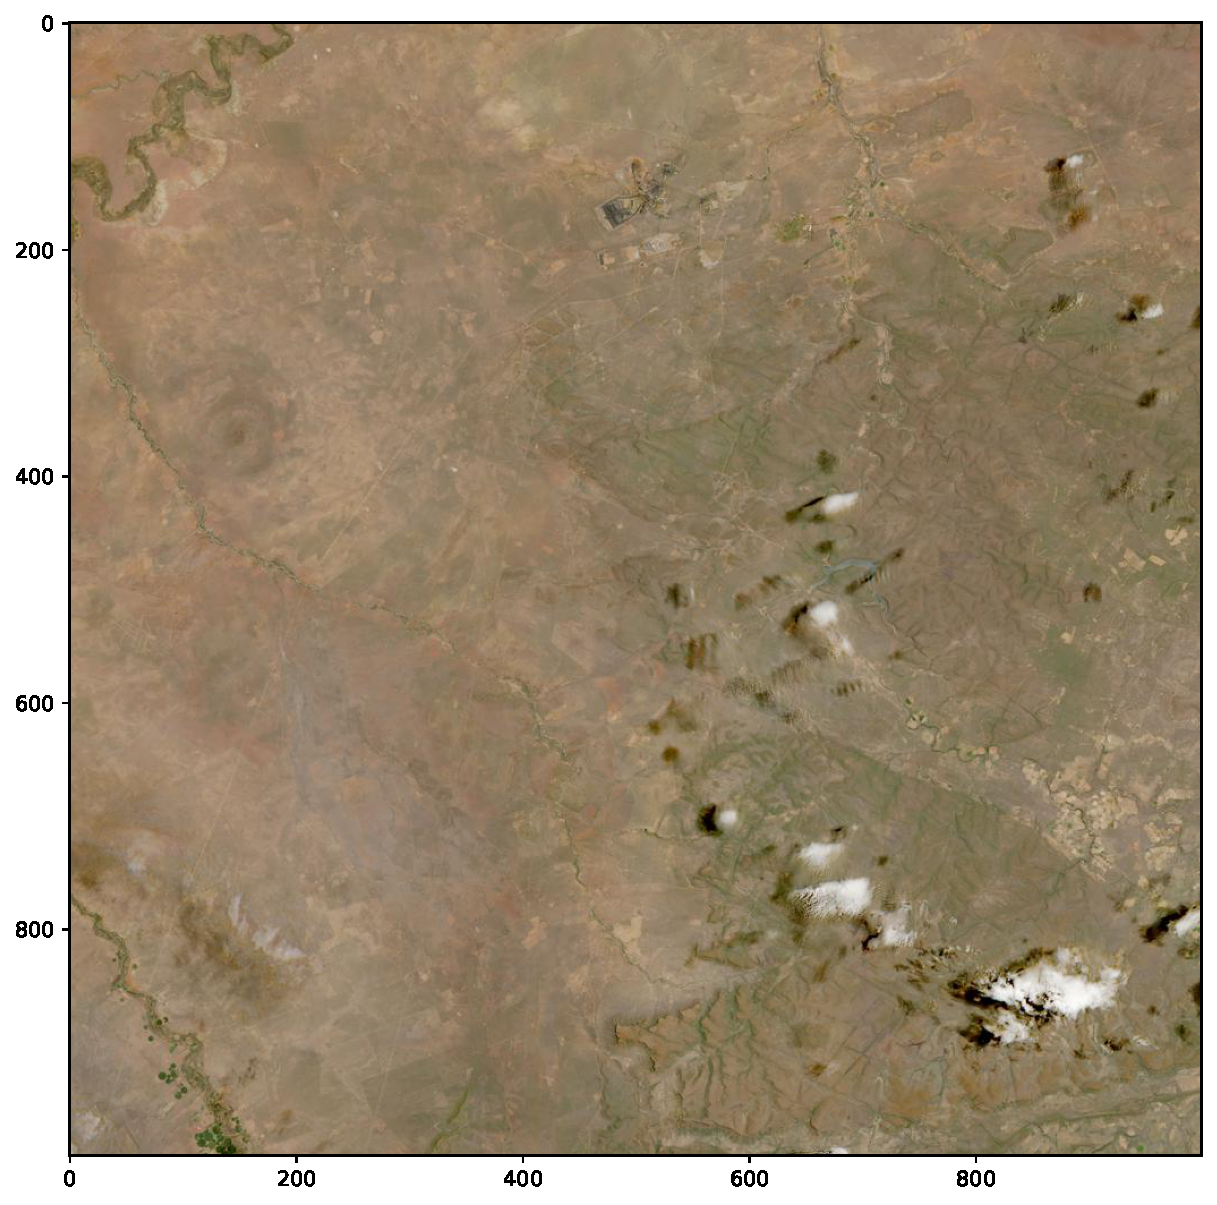
\includegraphics{Navigate_CMR_STAC_files/figure-pdf/cell-21-output-1.pdf}

\hypertarget{congrats-you-have-visualized-your-first-cloud-native-hls-asset}{%
\subsubsection{Congrats! You have visualized your first Cloud-Native HLS
asset!}\label{congrats-you-have-visualized-your-first-cloud-native-hls-asset}}

\end{document}
